\begin{frame}
    \frametitle{Точность полученного расписания}
    \begin{columns}
        \begin{column}{0.5\textwidth}
            \begin{figure}
                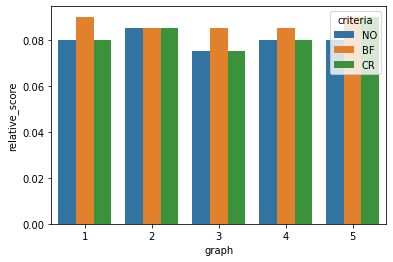
\includegraphics[width=\textwidth]{imgs/relative_score.png}
            \end{figure}
        \end{column}
        \begin{column}{0.5\textwidth}
            \begin{table}
                \caption*{Наборы исходных данных, используемых в тестировании}
                \begin{tabular}{c | c | c | c}
                    Граф & Вершин & Процессоров & Передач \\
                    \hline
                    1    & 126    & 4           & 716     \\
                    2    & 417    & 8           & 2367    \\
                    3    & 408    & 8           & 8763    \\
                    4    & 296    & 8           & 395     \\
                    5    & 93     & 4           & 92      \\
                \end{tabular}
            \end{table}
            % \begin{enumerate}
            %     \item 126 вершин, 4 процессора, 716 передач данных
            %     \item 417 вершин, 8 процессоров, 2367 передач данных
            %     \item 408 вершин, 8 процессоров, 8763 передач данных
            %     \item 396 вершин, 8 процессоров, 395 передачи данных
            %     \item 93 вершины, 4 процессора, 92 передачи данных
            % \end{enumerate}
        \end{column}
    \end{columns}

    \begin{equation*}
        relative\_score = \frac{\text{время полученного расписания}}{\text{время оптимального расписания}} - 1
    \end{equation*}
\end{frame}

\begin{frame}
    \frametitle{Время выполнения расписания}
    \begin{figure}
        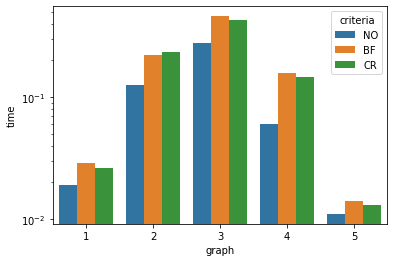
\includegraphics[width=0.7\textwidth]{imgs/times.png}
    \end{figure}
\end{frame}